\documentclass[a4paper,10pt,titlepage]{article}

\usepackage{geometry}
\usepackage{amsmath}
\usepackage{amssymb}
\usepackage{txfonts}
\usepackage{microtype}
\usepackage{epsfig}
\usepackage{graphicx}
\usepackage{moreverb}
\usepackage{hyperref}
\usepackage{listings}
\usepackage{xcolor}
\usepackage{textcomp}
\definecolor{listinggray}{gray}{0.98}
\definecolor{lbcolor}{rgb}{0.98,0.98,0.98}
\lstset{
	backgroundcolor=\color{lbcolor},
	tabsize=4,
	rulecolor=,
	language=matlab,
    basicstyle=\scriptsize\ttfamily,
    upquote=true,
    aboveskip={1.5\baselineskip},
    columns=fixed,
    showstringspaces=false,
    extendedchars=true,
    breaklines=true,
    prebreak = \raisebox{0ex}[0ex][0ex]{\ensuremath{\hookleftarrow}},
    frame=single,
    showtabs=false,
    showspaces=false,
    showstringspaces=false,
    identifierstyle=\ttfamily,
    keywordstyle=\color[rgb]{0,0,1},
    commentstyle=\color[rgb]{0.133,0.545,0.133},
    stringstyle=\color[rgb]{0.627,0.126,0.941},
}
\usepackage{eso-pic}
\usepackage{ifthen}

\AddToShipoutPictureBG{\ifthenelse{\equal{\value{page}}{0}}{}{
\includegraphics{template_files/backgroundlines}}}

\usepackage{units}
%\usepackage[T1]{fontenc}
%\usepackage[utf8]{inputenc}
\usepackage{physics}

\newcommand{\ee}{\mathrm{e}}
\newcommand{\ii}{\mathrm{i}}

\title{H1b: MD simulation -- dynamic properties}
\author{Andr\'eas Sundstr\"om and Linnea Hesslow}
\date{\today}

\begin{document}

\newgeometry{top=2cm,bottom=2cm,left=2cm,right=2cm}

\begin{titlepage}

\setcounter{page}{0}

\begin{center}
{\huge \bf \color{red} NB: The graded, first version of the report must be
                           returned if you hand in a second time! } \\
\vspace{3cm}
\makeatletter
{ \huge \@title } \\
\vspace{1cm}
{ \Large \@author }\\
\vspace{1cm}
{ \Large \@date }\\
\makeatother
\end{center}

\vfill

\begin{flushright}
{\Large
\begin{tabular}{|c|c|c|}
\hline
Task N\textsuperscript{\underline{o}} & Points & Avail.\ points \\ \hline
\hspace{3cm} & \hspace{3cm} & \hspace{3cm} \\ \hline
~ & ~ & ~ \\ \hline
~ & ~ & ~ \\ \hline
~ & ~ & ~ \\ \hline
~ & ~ & ~ \\ \hline
~ & ~ & ~ \\ \hline
~ & ~ & ~ \\ \hline
~ & ~ & ~ \\ \hline
$\sum$ & ~ & ~ \\
\hline
\end{tabular}}
\end{flushright}

\end{titlepage}

\newgeometry{top=2cm,bottom=2cm,left=1.5cm,right=7.4cm}


\section*{Introduction}

Already in antiquity people studied the effect of particles impinging on other
particles. Since then the art has developed \ldots\
(\emph{If you like to do so, you may take the opportunity to put the  methods
in a wider perspective here.}) Here is a random reference.\cite{lamport94}

\section*{Task 1}
We determined the theoretical lattice parameter ....

Figure~\ref{fig1} shows the potential energy as a function of the lattice parameter. We used a quadratic fit to find the minimum energy, and obtained $V_{\rm eq} \approx \unit[65.38]{\AA^3}$. This corresponds to the equilibrium lattice parameter $a_{\rm eq} \approx \unit[4.029]{\AA}$ at \unit[0]{K}, which we took as the initial lattice parameter for the following tasks.  

\begin{figure}[!ht]
\begin{center}
  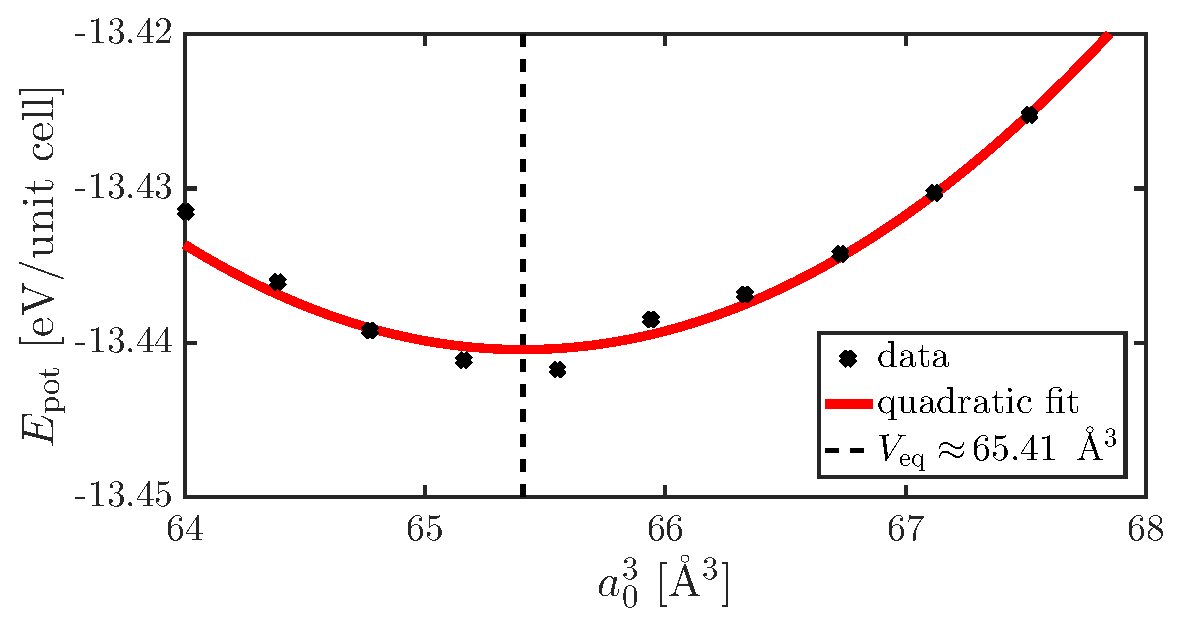
\includegraphics[width=0.7\textwidth]{../figures/potential_energy} 
  \caption{The potential energy per unit cell for aluminum as a function of the lattice parameter cubed.}
  \label{fig1}
\end{center}
\end{figure}

We find that figure~\ref{fig1} looks similar to the figure~1 in the homework problem file. 

\section*{Task 5}
Equation (82) in MD lecture notes:


\begin{align}
\Delta_{\rm MSD}(t) &= \lim_{T \rightarrow \infty} \frac{1}{T} \int_0^{T} d t' \frac{1}{N_{\rm atoms}} \sum_{i=0}^{N_{\rm atoms}-1} \left[{\bf r}_i(t+t') - {\bf r}_i(t') \right]^2 \\ &\Rightarrow \nonumber
\\
\Delta_{\rm MSD}(t_k) &\approx
\frac{1}{N_T -k}\frac{1}{N_{\rm atoms}} \sum_{j=0}^{N_T-k-1} \sum_{i=0}^{N_{\rm atoms}-1} \left[{\bf r}_i(t_{k+j}) - {\bf r}_i(t_j) \right]^2 
\end{align}

To determine M, we used mean of ... for t  > ...


\section*{Task 7}



The average ``power'' content in avariable , $X(t')$, at
some time, $t$, during some range of time, $T$, can be defined as
\begin{equation}
P_X(t,T) = \frac{1}{T}\int_{t-T/2}^{t+T/2}\dd{t'}\,X^2(t').
\end{equation}
This quantity can (in physically relevant systems) also be defined for
the process over all,
\begin{equation}
P_X = \lim_{T\to\infty} P_X(T)
= \lim_{T\to\infty} \frac{1}{T} \ev{\int_{0}^{T}\dd{t'}\,X^2(t')}.
\end{equation}
At this stage, we can introduce a 
We have the Fourier transform
\begin{equation}
\hat{f}(\omega) = \int_{-\infty}^{\infty}\dd{t} f(t)\ee^{\ii\omega t},
\end{equation}


Using these two functions, we can define a power spectrum
\begin{equation}
\begin{aligned}
\hat{P}(\omega) =& \ev{\abs{\hat{\vb*v}(\omega)}^2}_{\rm A}
=\ev{\hat{\vb*v}(\omega)\vdot \bar{\hat{\vb*v}}(\omega)}_{\rm A}\\
=& \ev{\int_{-\infty}^{\infty}\dd{t}\, \vb*v(t)\ee^{\ii\omega t}
  \int_{-\infty}^{\infty}\dd{t'}\, \vb*v(t')\ee^{-\ii\omega t'} }_{\rm A},
\end{aligned}
\end{equation}
where $\bar{\hat{\vb*v}}$ denotes the complex conjugate of
$\bar{\vb*v}$. We can now change varaibles to $t=t'+\tau$ and note
that the atom averages only falls on the velocities, which gives
\begin{equation}
\begin{aligned}
\hat{P}(\omega) 
=& \int_{-\infty}^{\infty}\dd\tau\, \ee^{\ii\omega\tau}
  \int_{-\infty}^{\infty}\dd{t'} \ev{\vb*v(t'+\tau)\vdot\vb*v(t') }_{\rm A},
\end{aligned}
\end{equation}







\section*{Problem 1}
As a starting point we first look at scattering from a hard-sphere
potential. We also consider the Lennard--Jones potential, which is depicted
in Figure~\ref{fig11}. (\emph{Always refer to Figures in the text.})

\begin{figure}[!ht]
\begin{center}
  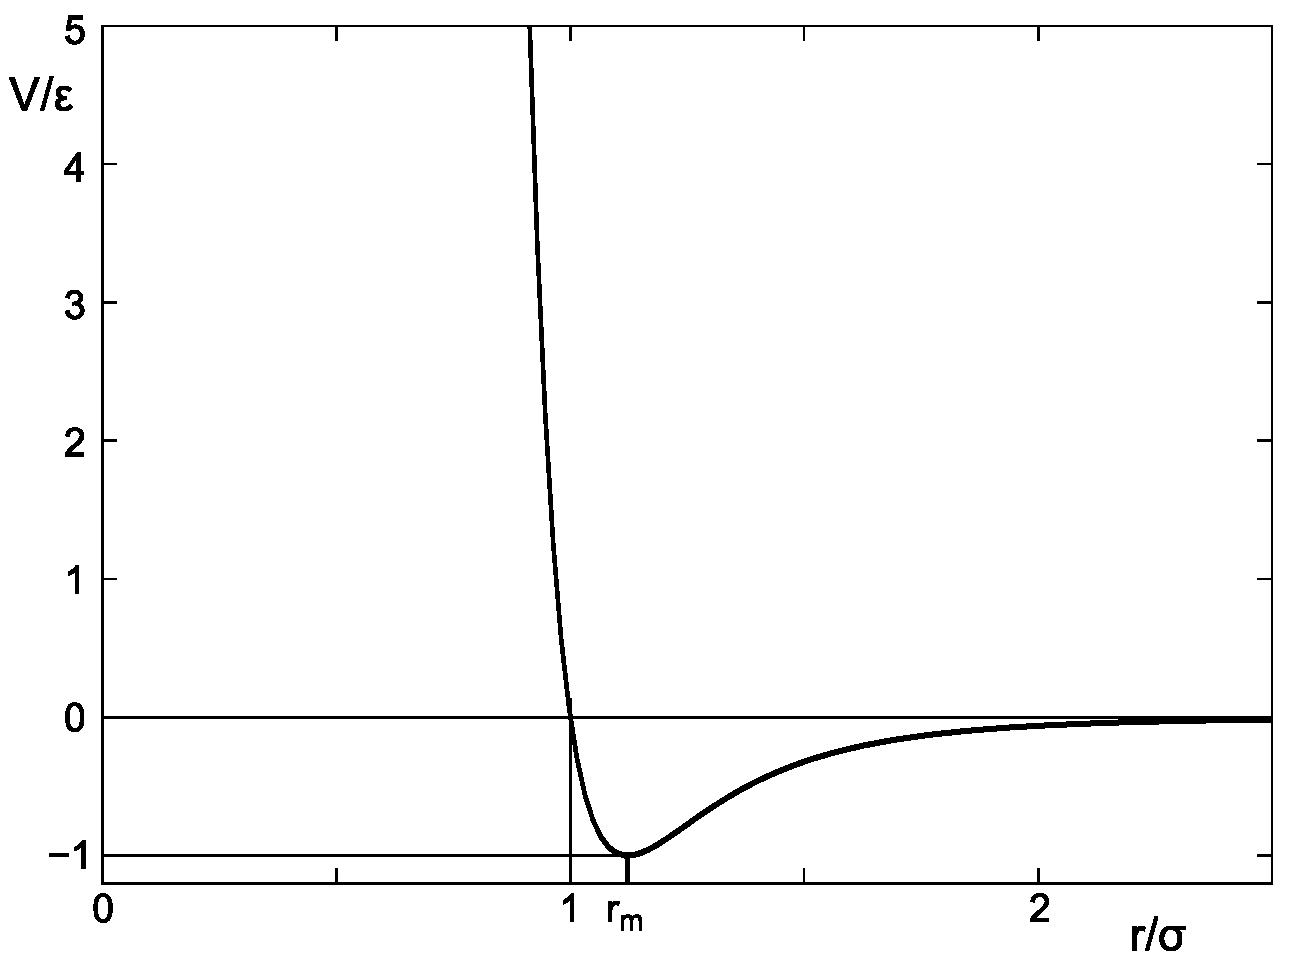
\includegraphics[width=0.7\textwidth]{template_files/LJ} 
  \caption{The Lennard--Jones potential.
  Make sure you label and have units on all axes! Also make sure that labels etc.\
  are legible and that, if you print in black and white, that you use different line
  styles when required to differentiate between curves. In \textsc{matlab}
  you can export any figure to an .eps file from File $\rightarrow$
  Export\ldots\ in the Figure window.}
  \label{fig1}
\end{center}
\end{figure}
  
\section*{Problem 2}

In the following we give an example of how to produce a table.
Use the code for Table~\ref{tab1} as a template.

\begin{table}[!ht]
  \begin{center}
    \caption{A dummy table}
    \begin{tabular}{l|c|c}\hline\hline
      \textbf{Col.~1} & \textbf{Col.~2} & \textbf{Col.~3} \\ \hline
      the & quick & brown \\ 
      fox & jumps & over \\ 
      the & lazy  & dog \\ 
      \hline\hline
    \end{tabular}
    \label{tab1}
  \end{center}
\end{table}

\section*{Problem 3}

If you find some part of the code particularly interesting you may 
include it in the text, otherwise it should be included in the appedix.
If you do want to include code the following commands will print
the text directly, with no \LaTeX~commands executed:

\begin{lstlisting}[language=matlab]
% Hello world ten times in MATLAB
for i = 1 : 10
  fprintf('Hello world %d!\n',i);
end
\end{lstlisting}

\begin{lstlisting}[language=python]
# Hello world ten times in Python
for i in range(10):
  print 'Hello world %d!' % i
\end{lstlisting}

\section*{Problem 4}
At some point it may be appropriate to include equations. It is done in the
following way:

\begin{equation}
  V(r) = 4\epsilon \left[ \left( \frac{\sigma}{r} \right)^{12} - 
    \left(\frac{\sigma}{r} \right)^{6} \right]
\end{equation}

Do number and reference all your equations.

\section*{Concluding discussion}

Use your favourite flavor of \LaTeX{} to compile the file:
\begin{verbatim}
xelatex template.tex
pdflatex template.tex
latex template.tex
\end{verbatim}
should all work.
If you use \verb+pdflatex+ or \verb+xelatex+, included figures need to be in
\verb+pdf+, \verb+jpg+, or \verb+png+ format. If you want to include eps
figures, you can easily convert them to \verb+pdf+ using the command
\begin{verbatim}
ps2pdf -dEPSCrop figure.eps figure.pdf
\end{verbatim}

\begin{thebibliography}{69}
\bibitem{lamport94} Leslie Lamport, \emph{\LaTeX: A Document Preparation
System}. Addison Wesley, Massachusetts, 2nd Edition, 1994.
\end{thebibliography}

\newpage

\appendix

\section{Source Code}

Include all source code here in the appendix. Keep the code formatting clean,
use indentation, and comment your code to make it easy to understand. Also,
break lines that are too long. (Keep them under 80 characters!)

%\subsection{Calculating pi using matlab: \texttt{pi.m}}
%\lstinputlisting[language=matlab,numbers=left]{template_files/pi.m}

%\subsection{Calculating pi using python: \texttt{pi.py}}
%\lstinputlisting[language=python,numbers=left]{template_files/pi.py}

\subsection{Main program task 1: \texttt{main\_T1.c}}
\lstinputlisting[language=c,numbers=left]{../code/main_T1.c}

\subsection{Main program  Task 2: \texttt{main\_T2.c}}
\lstinputlisting[language=c,numbers=left]{../code/main_T2.c}

\subsection{Temperature and pressure equilibration for tasks 3-7 : \texttt{main\_T3.c}}
\lstinputlisting[language=c,numbers=left]{../code/main_T3.c}

\subsection{Production runs for tasks 3-7 : \texttt{main\_Prod.c}}
\lstinputlisting[language=c,numbers=left]{../code/main_Prod.c}

\subsection{Production runs for tasks 3-7 : \texttt{main\_Prod.c}}
\lstinputlisting[language=c,numbers=left]{../code/main_Prod.c}


\subsection{Misc functions : \texttt{funcs.c}}
\lstinputlisting[language=c,numbers=left]{../code/funcs.c}

\section{Auxiliary }
\subsection{Makefile}
\lstinputlisting[language=bash,numbers=left]{../code/Makefile}



\section{Matlab scripts}
\subsection{Analysis scripts for tasks 3-7: \texttt{Al\_energies.m}}
\lstinputlisting[language=matlab,numbers=left]{../m_scripts/Al_energies.m}

\subsection{Improve figure appearance: \texttt{ImproveFigureCompPhys.m}}
\lstinputlisting[language=matlab,numbers=left]{../m_scripts/ImproveFigureCompPhys.m}

\subsection{Change size of figures: \texttt{setFigureSize.m}}
\lstinputlisting[language=matlab,numbers=left]{../m_scripts/setFigureSize.m}
\end{document}

%%% Local Variables:
%%% mode: latex
%%% TeX-master: t
%%% End:
